
\subsection*{What is a Procedure}
\begin{frame}{\textbf{What is a Procedure}}
    \begin{itemize}
        \item Procedures are "programs within programs"
        \item Procedures have their own environment
    \end{itemize}
    \begin{alertblock}{Functions vs. Procedures}
        \begin{equation}
            \text{Functions} \neq \text{Procedures}
        \end{equation}
        Functions are expressions, procedures are statements.\\
        Very often same implementation.
    \end{alertblock}
\end{frame}

\subsection*{Anatomy of a procedure}
\begin{frame}{\textbf{Anatomy of a Procedure}}
    \begin{figure}
        \lstinputlisting[language=Pascal]{examples/anatomy.pipl}
    \end{figure}
    \begin{block}{Params}
        \begin{itemize}
            \item \textbf{OBS} - "read only"
            \item \textbf{UPD} - "read/write"
            \item \textbf{OUT} - "write only"
        \end{itemize}
    \end{block}
\end{frame}

\begin{frame}{\textbf{Declaration vs. Calling}}
    \begin{figure}
        \lstinputlisting[language=pascal, basicstyle=\ttfamily\tiny]{examples/ex1.pipl}
        \label{fig:ex1}
        \caption{Swap Procedure}
    \end{figure}
\end{frame}

\subsection*{Paramter Semantics}
\begin{frame}{\textbf{Parameter Semantics}}
    \Large
    Two types of parameter semantics:
    \begin{itemize}
        \item Reference semantics
        \item Copy semantics
    \end{itemize}
\end{frame}

\begin{frame}{\textbf{Reference Semantics}}
    \Large
    \begin{itemize}
        \item Parameters become aliased to arguments 
        \item Points to same memory address
        \item Unsafe, but sometimes useful
    \end{itemize}
\end{frame}
\begin{frame}{\textbf{Running a procedure with reference semantics}}
    \Large
    \begin{enumerate}[<+->]
        \item Get stackframe
        \item Wipe environment
        \item Add parameters to the environment with same address as arg
        \item run the procedure code
        \item restore the environment
    \end{enumerate}
\end{frame}
\begin{frame}{\textbf{Copy Semantics}}
    \Large
    \begin{itemize}
        \item Parameters are declared as variables and initialized with args' value
        \item Safer
        \item More intuitive behavior
        \item More complicated to implement
    \end{itemize}
\end{frame}

\begin{frame}{\textbf{Running a procedure with copy semantics}}
    
    \begin{enumerate}[<+->]
        \item Get stackframe
        \item Get values of args
        \item Wipe environment
        \item Add parameters to environment
        \item init those parameters with the arg values
        \item run the procedure code
        \item get the values of the parameters
        \item restore the environment
        \item copy the parameter values back to the args
    \end{enumerate}
\end{frame}


\subsection*{Example!}
\begin{frame}{\textbf{Swap example v2}}
    \lstinputlisting[language=Pascal]{examples/paramater semantics/paramsem.pipl}
\end{frame}

\subsection*{Reference semantics!}
\begin{frame}\textbf{{Reference semantics}}
    \lstinputlisting[language=Pascal]{examples/paramater semantics/reference/paramsem.pipl}
\end{frame}

\begin{frame}\textbf{{Reference semantics}}
    \lstinputlisting[language=Pascal]{examples/paramater semantics/reference/paramsem1.pipl}
\end{frame}
\begin{frame}\textbf{{Reference semantics}}
    \lstinputlisting[language=Pascal]{examples/paramater semantics/reference/paramsem2.pipl}
\end{frame}
\begin{frame}\textbf{{Reference semantics}}
    \lstinputlisting[language=Pascal]{examples/paramater semantics/reference/paramsem3.pipl}
\end{frame}


\subsection*{Copy semantics!}
\begin{frame}\textbf{{Copy semantics}}
    \lstinputlisting[language=Pascal]{examples/paramater semantics/copy/paramsem.pipl}
\end{frame}
\begin{frame}\textbf{{Copy semantics}}
    \lstinputlisting[language=Pascal]{examples/paramater semantics/copy/paramsem1.pipl}
\end{frame}
\begin{frame}\textbf{{Copy semantics}}
    \lstinputlisting[language=Pascal]{examples/paramater semantics/copy/paramsem2.pipl}
\end{frame}
\begin{frame}\textbf{{Copy semantics}}
    \lstinputlisting[language=Pascal]{examples/paramater semantics/copy/paramsem3.pipl}
\end{frame}

%\section*{Slutt}
\subsection*{Q\&A}
\begin{frame}{Questions?}
    \begin{figure}
        \centering
        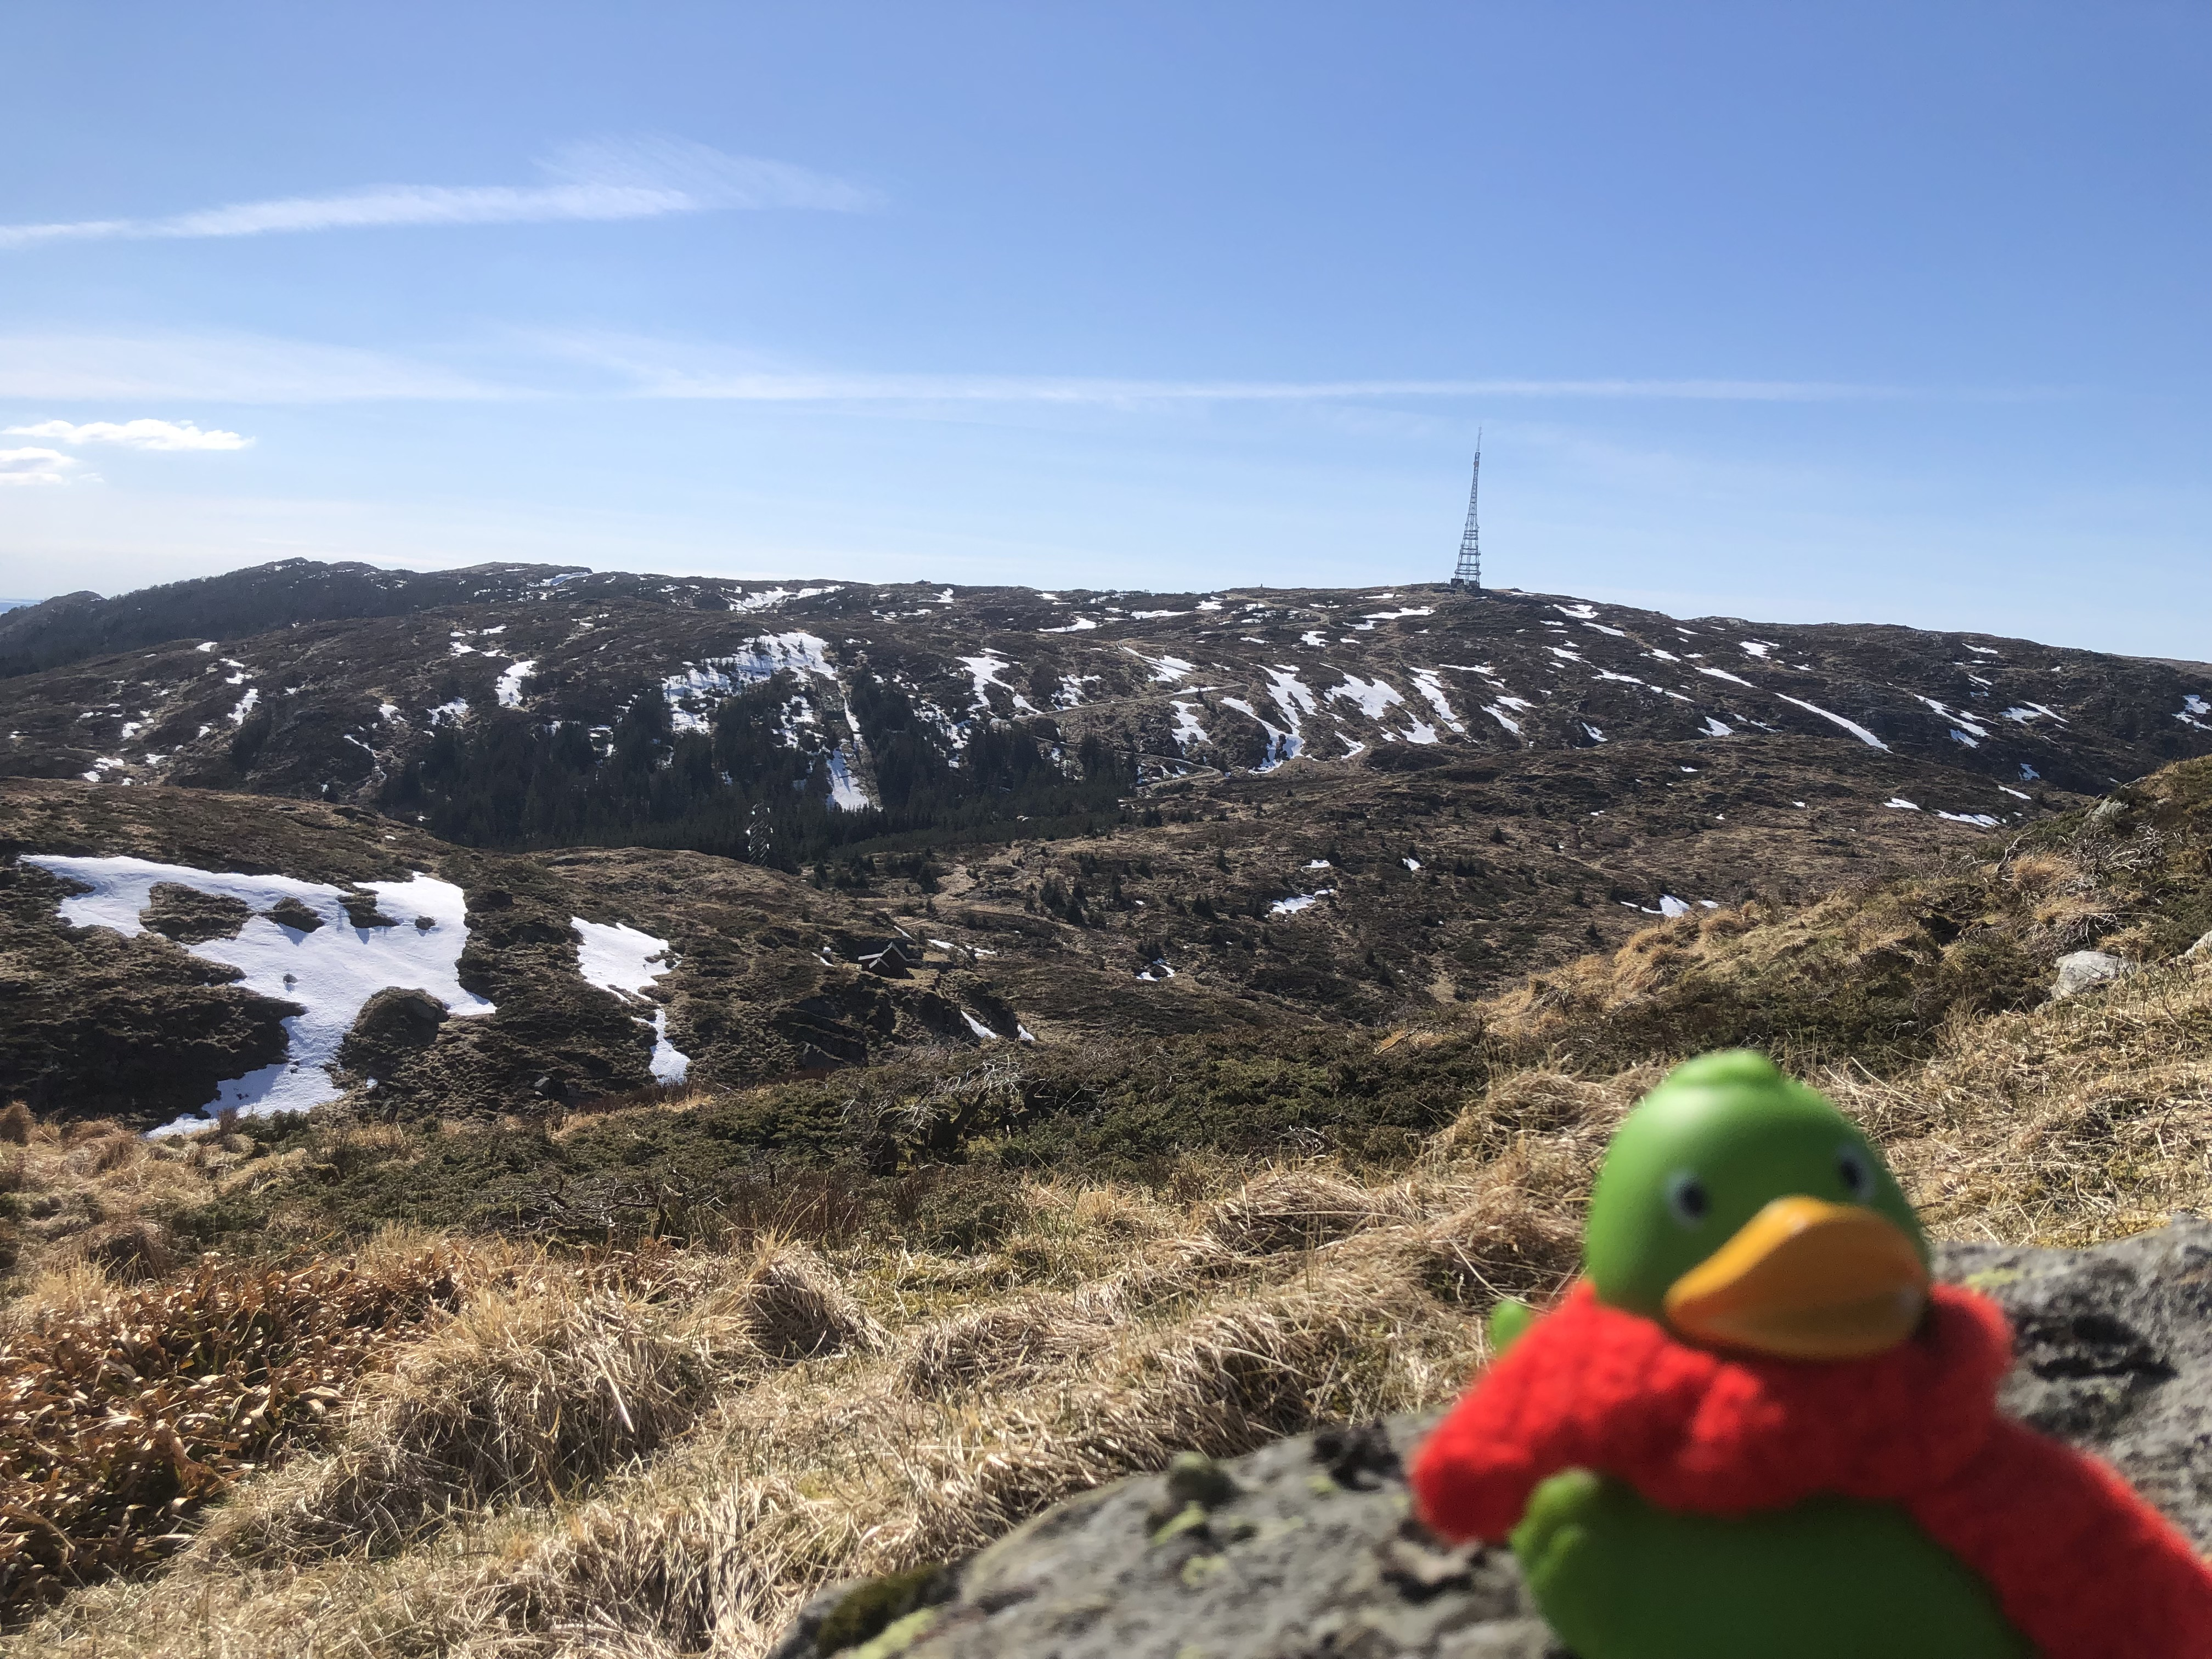
\includegraphics[height = 4.9cm]{guillaume5.jpg}
    \end{figure}
\end{frame}